\documentclass[11pt,aspectratio=169]{beamer}
% =============================================================================
%  Shared Beamer preamble — Machine Learning I & II, PEU-CD 2026 (ENEI / INEI)
%
%  Inherited from the ML_Foundations deck (Alexander Quispe), with three changes:
%    * `minted` removed — it shells out to Pygments and does not build under
%      tectonic; every code block in the course uses `listings`.
%    * unused packages (lipsum, blindtext, multimedia, videoframe) dropped.
%    * `bbm` dropped — its fonts are PK-only and tectonic cannot render them;
%      the indicator uses \mathbf{1} instead.
%    * a math-macro block added so all twelve lectures share one notation.
%
%  Each lecture is a standalone document:
%      \documentclass[11pt,aspectratio=169]{beamer}
%      % =============================================================================
%  Shared Beamer preamble — Machine Learning I & II, PEU-CD 2026 (ENEI / INEI)
%
%  Inherited from the ML_Foundations deck (Alexander Quispe), with three changes:
%    * `minted` removed — it shells out to Pygments and does not build under
%      tectonic; every code block in the course uses `listings`.
%    * unused packages (lipsum, blindtext, multimedia, videoframe) dropped.
%    * `bbm` dropped — its fonts are PK-only and tectonic cannot render them;
%      the indicator uses \mathbf{1} instead.
%    * a math-macro block added so all twelve lectures share one notation.
%
%  Each lecture is a standalone document:
%      \documentclass[11pt,aspectratio=169]{beamer}
%      % =============================================================================
%  Shared Beamer preamble — Machine Learning I & II, PEU-CD 2026 (ENEI / INEI)
%
%  Inherited from the ML_Foundations deck (Alexander Quispe), with three changes:
%    * `minted` removed — it shells out to Pygments and does not build under
%      tectonic; every code block in the course uses `listings`.
%    * unused packages (lipsum, blindtext, multimedia, videoframe) dropped.
%    * `bbm` dropped — its fonts are PK-only and tectonic cannot render them;
%      the indicator uses \mathbf{1} instead.
%    * a math-macro block added so all twelve lectures share one notation.
%
%  Each lecture is a standalone document:
%      \documentclass[11pt,aspectratio=169]{beamer}
%      \input{../../../style/preamble}
% =============================================================================

% ---------- fonts ----------
\usepackage{helvet}
\usepackage[default]{lato}
\usepackage{tgbonum}
\usepackage{mathpazo}
\usepackage[utf8]{inputenc}

% ---------- math ----------
\usepackage{amsmath,amssymb}
\usepackage{mathtools}

% ---------- graphics, tables, layout ----------
\usepackage{graphicx}
\usepackage{tikz}
\usetikzlibrary{positioning,calc,arrows,arrows.meta,decorations.markings,shapes.misc,matrix,shapes,fit}
\usepackage{array}
\usepackage{booktabs}
\usepackage{multirow}
\usepackage{dcolumn}
\usepackage{subcaption}
\usepackage{caption}
\usepackage{changepage}
\usepackage{xspace}
\usepackage{tcolorbox}
\tcbuselibrary{skins,breakable}
\usepackage[ruled,vlined]{algorithm2e}
\usepackage{listings}
\usepackage{appendixnumberbeamer}
\usepackage{hyperref}

\newcolumntype{d}[0]{D{.}{.}{5}}
\setbeamertemplate{caption}[numbered]

% ---------- palette (Okabe–Ito, colour-blind safe) ----------
\definecolor{blue}{RGB}{0,114,178}
\definecolor{red}{RGB}{213,94,0}
\definecolor{yellow}{RGB}{240,228,66}
\definecolor{green}{RGB}{0,158,115}
\definecolor{MyBackground}{RGB}{255,253,218}

\hypersetup{colorlinks=true, linkbordercolor={white}, linkcolor={blue}, urlcolor={blue}}

% ---------- beamer look ----------
\setbeamercolor{frametitle}{fg=blue}
\setbeamercolor{title}{fg=black}
\setbeamertemplate{footline}[frame number]
\setbeamertemplate{navigation symbols}{}
\setbeamertemplate{itemize items}{-}
\setbeamercolor{itemize item}{fg=blue}
\setbeamercolor{itemize subitem}{fg=blue}
\setbeamercolor{enumerate item}{fg=blue}
\setbeamercolor{enumerate subitem}{fg=blue}
\setbeamercolor{button}{bg=MyBackground,fg=blue}
\setbeamercolor{section in toc}{fg=blue}
\setbeamercolor{subsection in toc}{fg=red}
\setbeamersize{text margin left=1em,text margin right=1em}
\setbeamercolor{block title}{fg=white,bg=blue}
\setbeamercolor{block body}{bg=blue!5}
\setbeamercolor{block title alerted}{fg=white,bg=red}
\setbeamercolor{block body alerted}{bg=red!5}
\setbeamercolor{block title example}{fg=white,bg=green}
\setbeamercolor{block body example}{bg=green!5}
\setbeamertemplate{blocks}[rounded][shadow=false]

\newenvironment{wideitemize}{\itemize\addtolength{\itemsep}{10pt}}{\enditemize}

\newenvironment{transitionframe}{
  \setbeamercolor{background canvas}{bg=yellow}
  \begin{frame}}{
  \end{frame}
}

% Section divider: a plain frame with a large blue title.
\newcommand{\sectionframe}[1]{%
  \section{#1}%
  \begin{frame}[plain]\vfill\begin{center}{\Huge\textcolor{blue}{#1}}\end{center}\vfill\end{frame}}

% ---------- proof / derivation environments ----------
% derivation: a boxed, step-by-step algebraic argument. Title is the claim.
\newtcolorbox{derivation}[1]{enhanced, colback=blue!3, colframe=blue, fonttitle=\bfseries,
  title={#1}, boxrule=0.6pt, left=4pt, right=4pt, top=3pt, bottom=3pt, arc=2pt}
% claim: a result to be proved (theorem / lemma / proposition).
\newtcolorbox{claim}[1]{enhanced, colback=white, colframe=black, fonttitle=\bfseries,
  title={#1}, boxrule=0.6pt, left=4pt, right=4pt, top=3pt, bottom=3pt, arc=2pt}
% keypoint: the one line to remember from a slide.
\newtcolorbox{keypoint}{enhanced, colback=green!6, colframe=green, boxrule=0.6pt,
  left=4pt, right=4pt, top=3pt, bottom=3pt, arc=2pt}
% caution: a common mistake or a subtlety.
\newtcolorbox{caution}{enhanced, colback=red!5, colframe=red, boxrule=0.6pt,
  left=4pt, right=4pt, top=3pt, bottom=3pt, arc=2pt}

% ---------- code ----------
\lstset{
  basicstyle=\ttfamily\scriptsize, keywordstyle=\color{blue}\bfseries,
  commentstyle=\color{green}, stringstyle=\color{red},
  showstringspaces=false, breaklines=true, frame=single, rulecolor=\color{black!30},
  numbers=none, xleftmargin=4pt, framexleftmargin=4pt, language=Python
}

\input{../../../style/macros}

% ---------- course-wide title metadata ----------
\newcommand{\courseinstitution}{ENEI -- INEI \,\textperiodcentered\, PEU-CD 2026}
\newcommand{\courseauthor}{Alexander Quispe}
\institute{\courseinstitution}
\author{\courseauthor}

% =============================================================================

% ---------- fonts ----------
\usepackage{helvet}
\usepackage[default]{lato}
\usepackage{tgbonum}
\usepackage{mathpazo}
\usepackage[utf8]{inputenc}

% ---------- math ----------
\usepackage{amsmath,amssymb}
\usepackage{mathtools}

% ---------- graphics, tables, layout ----------
\usepackage{graphicx}
\usepackage{tikz}
\usetikzlibrary{positioning,calc,arrows,arrows.meta,decorations.markings,shapes.misc,matrix,shapes,fit}
\usepackage{array}
\usepackage{booktabs}
\usepackage{multirow}
\usepackage{dcolumn}
\usepackage{subcaption}
\usepackage{caption}
\usepackage{changepage}
\usepackage{xspace}
\usepackage{tcolorbox}
\tcbuselibrary{skins,breakable}
\usepackage[ruled,vlined]{algorithm2e}
\usepackage{listings}
\usepackage{appendixnumberbeamer}
\usepackage{hyperref}

\newcolumntype{d}[0]{D{.}{.}{5}}
\setbeamertemplate{caption}[numbered]

% ---------- palette (Okabe–Ito, colour-blind safe) ----------
\definecolor{blue}{RGB}{0,114,178}
\definecolor{red}{RGB}{213,94,0}
\definecolor{yellow}{RGB}{240,228,66}
\definecolor{green}{RGB}{0,158,115}
\definecolor{MyBackground}{RGB}{255,253,218}

\hypersetup{colorlinks=true, linkbordercolor={white}, linkcolor={blue}, urlcolor={blue}}

% ---------- beamer look ----------
\setbeamercolor{frametitle}{fg=blue}
\setbeamercolor{title}{fg=black}
\setbeamertemplate{footline}[frame number]
\setbeamertemplate{navigation symbols}{}
\setbeamertemplate{itemize items}{-}
\setbeamercolor{itemize item}{fg=blue}
\setbeamercolor{itemize subitem}{fg=blue}
\setbeamercolor{enumerate item}{fg=blue}
\setbeamercolor{enumerate subitem}{fg=blue}
\setbeamercolor{button}{bg=MyBackground,fg=blue}
\setbeamercolor{section in toc}{fg=blue}
\setbeamercolor{subsection in toc}{fg=red}
\setbeamersize{text margin left=1em,text margin right=1em}
\setbeamercolor{block title}{fg=white,bg=blue}
\setbeamercolor{block body}{bg=blue!5}
\setbeamercolor{block title alerted}{fg=white,bg=red}
\setbeamercolor{block body alerted}{bg=red!5}
\setbeamercolor{block title example}{fg=white,bg=green}
\setbeamercolor{block body example}{bg=green!5}
\setbeamertemplate{blocks}[rounded][shadow=false]

\newenvironment{wideitemize}{\itemize\addtolength{\itemsep}{10pt}}{\enditemize}

\newenvironment{transitionframe}{
  \setbeamercolor{background canvas}{bg=yellow}
  \begin{frame}}{
  \end{frame}
}

% Section divider: a plain frame with a large blue title.
\newcommand{\sectionframe}[1]{%
  \section{#1}%
  \begin{frame}[plain]\vfill\begin{center}{\Huge\textcolor{blue}{#1}}\end{center}\vfill\end{frame}}

% ---------- proof / derivation environments ----------
% derivation: a boxed, step-by-step algebraic argument. Title is the claim.
\newtcolorbox{derivation}[1]{enhanced, colback=blue!3, colframe=blue, fonttitle=\bfseries,
  title={#1}, boxrule=0.6pt, left=4pt, right=4pt, top=3pt, bottom=3pt, arc=2pt}
% claim: a result to be proved (theorem / lemma / proposition).
\newtcolorbox{claim}[1]{enhanced, colback=white, colframe=black, fonttitle=\bfseries,
  title={#1}, boxrule=0.6pt, left=4pt, right=4pt, top=3pt, bottom=3pt, arc=2pt}
% keypoint: the one line to remember from a slide.
\newtcolorbox{keypoint}{enhanced, colback=green!6, colframe=green, boxrule=0.6pt,
  left=4pt, right=4pt, top=3pt, bottom=3pt, arc=2pt}
% caution: a common mistake or a subtlety.
\newtcolorbox{caution}{enhanced, colback=red!5, colframe=red, boxrule=0.6pt,
  left=4pt, right=4pt, top=3pt, bottom=3pt, arc=2pt}

% ---------- code ----------
\lstset{
  basicstyle=\ttfamily\scriptsize, keywordstyle=\color{blue}\bfseries,
  commentstyle=\color{green}, stringstyle=\color{red},
  showstringspaces=false, breaklines=true, frame=single, rulecolor=\color{black!30},
  numbers=none, xleftmargin=4pt, framexleftmargin=4pt, language=Python
}

% =============================================================================
%  Notation — one convention for all lectures
%
%  scalars      x, y, w           plain italic
%  vectors      \vx \vy \vw       bold lower-case
%  matrices     \vX \vW \vSigma   bold upper-case
%  parameters   \vbeta \vtheta    bold Greek
%  transpose    \vX\T             \top
% =============================================================================
\newcommand{\R}{\mathbb{R}}
\newcommand{\E}{\mathbb{E}}
\newcommand{\Prob}{\mathbb{P}}
\DeclareMathOperator{\Var}{Var}
\DeclareMathOperator{\Cov}{Cov}
\DeclareMathOperator{\tr}{tr}
\DeclareMathOperator{\diag}{diag}
\DeclareMathOperator{\rank}{rank}
\DeclareMathOperator{\sign}{sign}
\DeclareMathOperator{\col}{col}
\DeclareMathOperator{\RSS}{RSS}
\DeclareMathOperator*{\argmin}{arg\,min}
\DeclareMathOperator*{\argmax}{arg\,max}
\newcommand{\norm}[1]{\left\lVert #1 \right\rVert}
\newcommand{\abs}[1]{\left\lvert #1 \right\rvert}
\newcommand{\inner}[2]{\left\langle #1,\, #2 \right\rangle}
\newcommand{\ind}[1]{\mathbf{1}\!\left\{#1\right\}}
\newcommand{\T}{^{\top}}
\newcommand{\inv}{^{-1}}
\newcommand{\half}{\tfrac{1}{2}}
\newcommand{\eps}{\varepsilon}
\newcommand{\Dset}{\mathcal{D}}
\newcommand{\Hset}{\mathcal{H}}
\newcommand{\Lcal}{\mathcal{L}}
\newcommand{\Ncal}{\mathcal{N}}

% bold vectors
\newcommand{\vx}{\mathbf{x}}   \newcommand{\vy}{\mathbf{y}}   \newcommand{\vz}{\mathbf{z}}
\newcommand{\vw}{\mathbf{w}}   \newcommand{\vu}{\mathbf{u}}   \newcommand{\vv}{\mathbf{v}}
\newcommand{\vb}{\mathbf{b}}   \newcommand{\vh}{\mathbf{h}}   \newcommand{\vr}{\mathbf{r}}
\newcommand{\vc}{\mathbf{c}}   \newcommand{\vf}{\mathbf{f}}   \newcommand{\vg}{\mathbf{g}}
\newcommand{\vp}{\mathbf{p}}   \newcommand{\vq}{\mathbf{q}}   \newcommand{\vs}{\mathbf{s}}
\newcommand{\va}{\mathbf{a}}   \newcommand{\vd}{\mathbf{d}}   \newcommand{\vt}{\mathbf{t}}
\newcommand{\vk}{\mathbf{k}}   \newcommand{\vm}{\mathbf{m}}   \newcommand{\vn}{\mathbf{n}}
\newcommand{\vzero}{\mathbf{0}} \newcommand{\vone}{\mathbf{1}}
% bold matrices
\newcommand{\vX}{\mathbf{X}}   \newcommand{\vY}{\mathbf{Y}}   \newcommand{\vZ}{\mathbf{Z}}
\newcommand{\vW}{\mathbf{W}}   \newcommand{\vH}{\mathbf{H}}   \newcommand{\vI}{\mathbf{I}}
\newcommand{\vA}{\mathbf{A}}   \newcommand{\vB}{\mathbf{B}}   \newcommand{\vC}{\mathbf{C}}
\newcommand{\vD}{\mathbf{D}}   \newcommand{\vP}{\mathbf{P}}   \newcommand{\vQ}{\mathbf{Q}}
\newcommand{\vU}{\mathbf{U}}   \newcommand{\vV}{\mathbf{V}}   \newcommand{\vS}{\mathbf{S}}
\newcommand{\vM}{\mathbf{M}}   \newcommand{\vK}{\mathbf{K}}   \newcommand{\vG}{\mathbf{G}}
% bold Greek
\newcommand{\vbeta}{\boldsymbol{\beta}}     \newcommand{\valpha}{\boldsymbol{\alpha}}
\newcommand{\vtheta}{\boldsymbol{\theta}}   \newcommand{\vmu}{\boldsymbol{\mu}}
\newcommand{\vSigma}{\boldsymbol{\Sigma}}   \newcommand{\vLambda}{\boldsymbol{\Lambda}}
\newcommand{\veps}{\boldsymbol{\varepsilon}} \newcommand{\vphi}{\boldsymbol{\phi}}
\newcommand{\vgamma}{\boldsymbol{\gamma}}   \newcommand{\vlambda}{\boldsymbol{\lambda}}
\newcommand{\vdelta}{\boldsymbol{\delta}}   \newcommand{\vnu}{\boldsymbol{\nu}}
\newcommand{\vxi}{\boldsymbol{\xi}}         \newcommand{\vpi}{\boldsymbol{\pi}}
\newcommand{\vomega}{\boldsymbol{\omega}}



% ---------- course-wide title metadata ----------
\newcommand{\courseinstitution}{ENEI -- INEI \,\textperiodcentered\, PEU-CD 2026}
\newcommand{\courseauthor}{Alexander Quispe}
\institute{\courseinstitution}
\author{\courseauthor}

% =============================================================================

% ---------- fonts ----------
\usepackage{helvet}
\usepackage[default]{lato}
\usepackage{tgbonum}
\usepackage{mathpazo}
\usepackage[utf8]{inputenc}

% ---------- math ----------
\usepackage{amsmath,amssymb}
\usepackage{mathtools}

% ---------- graphics, tables, layout ----------
\usepackage{graphicx}
\usepackage{tikz}
\usetikzlibrary{positioning,calc,arrows,arrows.meta,decorations.markings,shapes.misc,matrix,shapes,fit}
\usepackage{array}
\usepackage{booktabs}
\usepackage{multirow}
\usepackage{dcolumn}
\usepackage{subcaption}
\usepackage{caption}
\usepackage{changepage}
\usepackage{xspace}
\usepackage{tcolorbox}
\tcbuselibrary{skins,breakable}
\usepackage[ruled,vlined]{algorithm2e}
\usepackage{listings}
\usepackage{appendixnumberbeamer}
\usepackage{hyperref}

\newcolumntype{d}[0]{D{.}{.}{5}}
\setbeamertemplate{caption}[numbered]

% ---------- palette (Okabe–Ito, colour-blind safe) ----------
\definecolor{blue}{RGB}{0,114,178}
\definecolor{red}{RGB}{213,94,0}
\definecolor{yellow}{RGB}{240,228,66}
\definecolor{green}{RGB}{0,158,115}
\definecolor{MyBackground}{RGB}{255,253,218}

\hypersetup{colorlinks=true, linkbordercolor={white}, linkcolor={blue}, urlcolor={blue}}

% ---------- beamer look ----------
\setbeamercolor{frametitle}{fg=blue}
\setbeamercolor{title}{fg=black}
\setbeamertemplate{footline}[frame number]
\setbeamertemplate{navigation symbols}{}
\setbeamertemplate{itemize items}{-}
\setbeamercolor{itemize item}{fg=blue}
\setbeamercolor{itemize subitem}{fg=blue}
\setbeamercolor{enumerate item}{fg=blue}
\setbeamercolor{enumerate subitem}{fg=blue}
\setbeamercolor{button}{bg=MyBackground,fg=blue}
\setbeamercolor{section in toc}{fg=blue}
\setbeamercolor{subsection in toc}{fg=red}
\setbeamersize{text margin left=1em,text margin right=1em}
\setbeamercolor{block title}{fg=white,bg=blue}
\setbeamercolor{block body}{bg=blue!5}
\setbeamercolor{block title alerted}{fg=white,bg=red}
\setbeamercolor{block body alerted}{bg=red!5}
\setbeamercolor{block title example}{fg=white,bg=green}
\setbeamercolor{block body example}{bg=green!5}
\setbeamertemplate{blocks}[rounded][shadow=false]

\newenvironment{wideitemize}{\itemize\addtolength{\itemsep}{10pt}}{\enditemize}

\newenvironment{transitionframe}{
  \setbeamercolor{background canvas}{bg=yellow}
  \begin{frame}}{
  \end{frame}
}

% Section divider: a plain frame with a large blue title.
\newcommand{\sectionframe}[1]{%
  \section{#1}%
  \begin{frame}[plain]\vfill\begin{center}{\Huge\textcolor{blue}{#1}}\end{center}\vfill\end{frame}}

% ---------- proof / derivation environments ----------
% derivation: a boxed, step-by-step algebraic argument. Title is the claim.
\newtcolorbox{derivation}[1]{enhanced, colback=blue!3, colframe=blue, fonttitle=\bfseries,
  title={#1}, boxrule=0.6pt, left=4pt, right=4pt, top=3pt, bottom=3pt, arc=2pt}
% claim: a result to be proved (theorem / lemma / proposition).
\newtcolorbox{claim}[1]{enhanced, colback=white, colframe=black, fonttitle=\bfseries,
  title={#1}, boxrule=0.6pt, left=4pt, right=4pt, top=3pt, bottom=3pt, arc=2pt}
% keypoint: the one line to remember from a slide.
\newtcolorbox{keypoint}{enhanced, colback=green!6, colframe=green, boxrule=0.6pt,
  left=4pt, right=4pt, top=3pt, bottom=3pt, arc=2pt}
% caution: a common mistake or a subtlety.
\newtcolorbox{caution}{enhanced, colback=red!5, colframe=red, boxrule=0.6pt,
  left=4pt, right=4pt, top=3pt, bottom=3pt, arc=2pt}

% ---------- code ----------
\lstset{
  basicstyle=\ttfamily\scriptsize, keywordstyle=\color{blue}\bfseries,
  commentstyle=\color{green}, stringstyle=\color{red},
  showstringspaces=false, breaklines=true, frame=single, rulecolor=\color{black!30},
  numbers=none, xleftmargin=4pt, framexleftmargin=4pt, language=Python
}

% =============================================================================
%  Notation — one convention for all lectures
%
%  scalars      x, y, w           plain italic
%  vectors      \vx \vy \vw       bold lower-case
%  matrices     \vX \vW \vSigma   bold upper-case
%  parameters   \vbeta \vtheta    bold Greek
%  transpose    \vX\T             \top
% =============================================================================
\newcommand{\R}{\mathbb{R}}
\newcommand{\E}{\mathbb{E}}
\newcommand{\Prob}{\mathbb{P}}
\DeclareMathOperator{\Var}{Var}
\DeclareMathOperator{\Cov}{Cov}
\DeclareMathOperator{\tr}{tr}
\DeclareMathOperator{\diag}{diag}
\DeclareMathOperator{\rank}{rank}
\DeclareMathOperator{\sign}{sign}
\DeclareMathOperator{\col}{col}
\DeclareMathOperator{\RSS}{RSS}
\DeclareMathOperator*{\argmin}{arg\,min}
\DeclareMathOperator*{\argmax}{arg\,max}
\newcommand{\norm}[1]{\left\lVert #1 \right\rVert}
\newcommand{\abs}[1]{\left\lvert #1 \right\rvert}
\newcommand{\inner}[2]{\left\langle #1,\, #2 \right\rangle}
\newcommand{\ind}[1]{\mathbf{1}\!\left\{#1\right\}}
\newcommand{\T}{^{\top}}
\newcommand{\inv}{^{-1}}
\newcommand{\half}{\tfrac{1}{2}}
\newcommand{\eps}{\varepsilon}
\newcommand{\Dset}{\mathcal{D}}
\newcommand{\Hset}{\mathcal{H}}
\newcommand{\Lcal}{\mathcal{L}}
\newcommand{\Ncal}{\mathcal{N}}

% bold vectors
\newcommand{\vx}{\mathbf{x}}   \newcommand{\vy}{\mathbf{y}}   \newcommand{\vz}{\mathbf{z}}
\newcommand{\vw}{\mathbf{w}}   \newcommand{\vu}{\mathbf{u}}   \newcommand{\vv}{\mathbf{v}}
\newcommand{\vb}{\mathbf{b}}   \newcommand{\vh}{\mathbf{h}}   \newcommand{\vr}{\mathbf{r}}
\newcommand{\vc}{\mathbf{c}}   \newcommand{\vf}{\mathbf{f}}   \newcommand{\vg}{\mathbf{g}}
\newcommand{\vp}{\mathbf{p}}   \newcommand{\vq}{\mathbf{q}}   \newcommand{\vs}{\mathbf{s}}
\newcommand{\va}{\mathbf{a}}   \newcommand{\vd}{\mathbf{d}}   \newcommand{\vt}{\mathbf{t}}
\newcommand{\vk}{\mathbf{k}}   \newcommand{\vm}{\mathbf{m}}   \newcommand{\vn}{\mathbf{n}}
\newcommand{\vzero}{\mathbf{0}} \newcommand{\vone}{\mathbf{1}}
% bold matrices
\newcommand{\vX}{\mathbf{X}}   \newcommand{\vY}{\mathbf{Y}}   \newcommand{\vZ}{\mathbf{Z}}
\newcommand{\vW}{\mathbf{W}}   \newcommand{\vH}{\mathbf{H}}   \newcommand{\vI}{\mathbf{I}}
\newcommand{\vA}{\mathbf{A}}   \newcommand{\vB}{\mathbf{B}}   \newcommand{\vC}{\mathbf{C}}
\newcommand{\vD}{\mathbf{D}}   \newcommand{\vP}{\mathbf{P}}   \newcommand{\vQ}{\mathbf{Q}}
\newcommand{\vU}{\mathbf{U}}   \newcommand{\vV}{\mathbf{V}}   \newcommand{\vS}{\mathbf{S}}
\newcommand{\vM}{\mathbf{M}}   \newcommand{\vK}{\mathbf{K}}   \newcommand{\vG}{\mathbf{G}}
% bold Greek
\newcommand{\vbeta}{\boldsymbol{\beta}}     \newcommand{\valpha}{\boldsymbol{\alpha}}
\newcommand{\vtheta}{\boldsymbol{\theta}}   \newcommand{\vmu}{\boldsymbol{\mu}}
\newcommand{\vSigma}{\boldsymbol{\Sigma}}   \newcommand{\vLambda}{\boldsymbol{\Lambda}}
\newcommand{\veps}{\boldsymbol{\varepsilon}} \newcommand{\vphi}{\boldsymbol{\phi}}
\newcommand{\vgamma}{\boldsymbol{\gamma}}   \newcommand{\vlambda}{\boldsymbol{\lambda}}
\newcommand{\vdelta}{\boldsymbol{\delta}}   \newcommand{\vnu}{\boldsymbol{\nu}}
\newcommand{\vxi}{\boldsymbol{\xi}}         \newcommand{\vpi}{\boldsymbol{\pi}}
\newcommand{\vomega}{\boldsymbol{\omega}}



% ---------- course-wide title metadata ----------
\newcommand{\courseinstitution}{ENEI -- INEI \,\textperiodcentered\, PEU-CD 2026}
\newcommand{\courseauthor}{Alexander Quispe}
\institute{\courseinstitution}
\author{\courseauthor}

\graphicspath{{figures/}}

\title{\textcolor{blue}{Lecture 4 \\ Decision Trees and Bagging}}
\subtitle{Machine Learning I}
\date{September 18, 2026}

\begin{document}

\begin{frame}[plain]
\maketitle
\end{frame}

\begin{frame}{Outline}
\tableofcontents
\end{frame}

\begin{frame}{A Different Hypothesis Class}
Three lectures on $\Hset_{\text{lin}}$. Its limitation is structural: a linear model cannot represent
\[
y=\ind{x_1>a\ \text{and}\ x_2<b},\qquad y=x_1\cdot x_2,\qquad y=\text{XOR}(x_1,x_2)
\]
without someone hand-crafting the right features. Trees learn the features.
\begin{center}
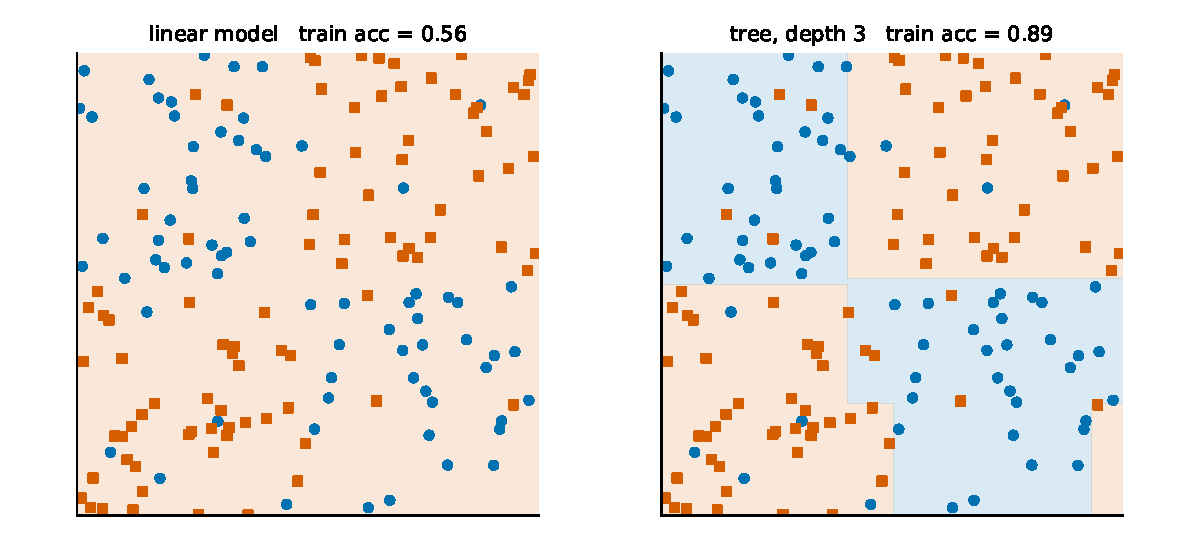
\includegraphics[height=0.5\textheight]{fig_tree_vs_linear.pdf}
\end{center}
\vspace{-4pt}
Same data. Left: the best line. Right: a depth-3 tree. The tree's boundary is a union of axis-aligned boxes.
\end{frame}

% =============================================================================
\sectionframe{Decision Trees}
% =============================================================================

\begin{frame}{The Function Class}
A binary decision tree partitions $\R^p$ into $M$ disjoint rectangles $R_1,\dots,R_M$ by asking one
question per internal node: \emph{is $x_j\le s$?} Each leaf $m$ carries a constant prediction $c_m$:
\[
f(\vx)=\sum_{m=1}^M c_m\,\ind{\vx\in R_m}.
\]
\begin{itemize}
  \item \textbf{Regression:} $c_m\in\R$. \quad \textbf{Classification:} $c_m\in\{1,\dots,K\}$, or a vector of class proportions.
  \item Piecewise constant. Discontinuous at every split. No parameters in the usual sense --- the ``parameters''
        are the questions and their order.
  \item Invariant to monotone transformations of any single feature: $\log x_j$ and $x_j$ produce the same tree.
        No standardization needed --- a first for this course.
\end{itemize}
\end{frame}

\begin{frame}{What Goes in a Leaf}\small
Given the partition, choose the $c_m$ to minimize empirical risk. The regions are disjoint, so this separates.
\begin{derivation}{Regression, squared loss}
\[
\hat c_m=\argmin_c\sum_{i:\,\vx_i\in R_m}(y_i-c)^2 ,\qquad
\frac{d}{dc}\sum_i(y_i-c)^2=-2\sum_i(y_i-c)=0
\]
\[
\Rightarrow\quad
\hat c_m=\frac{1}{N_m}\sum_{i:\,\vx_i\in R_m}y_i=\bar y_m .
\]
\end{derivation}
\begin{derivation}{Classification, 0/1 loss}
With $\hat p_{mk}=\frac1{N_m}\sum_{i\in R_m}\ind{y_i=k}$ the class proportions in the leaf,
\[
\hat c_m=\argmin_k\sum_{i\in R_m}\ind{y_i\ne k}=\argmin_k N_m(1-\hat p_{mk})=\argmax_k\hat p_{mk}.
\]
\end{derivation}
Leaves predict the mean (regression) or the majority (classification) of what fell into them.
The whole difficulty is in choosing the partition.
\end{frame}

\begin{frame}{How Many Trees Are There?}
Even with the leaf values settled, the search space is enormous:
\begin{itemize}
  \item A single split on feature $j$ with $N$ distinct values has $N-1$ candidate thresholds. With $p$ features:
        $p(N-1)$ candidate first questions.
  \item A tree of depth $d$ makes up to $2^d-1$ such choices, and the choices interact.
  \item Finding the smallest tree consistent with a dataset is NP-complete (Hyafil \& Rivest, 1976).
\end{itemize}
\vspace{6pt}
\begin{keypoint}
No algorithm finds the best tree. Every tree learner is \textbf{greedy}: pick the best single split now,
recurse, never look back. What ``best split'' means is the content of the next section.
\end{keypoint}
\end{frame}

% =============================================================================
\sectionframe{Impurity and Information Gain}
% =============================================================================

\begin{frame}{Measuring How Mixed a Node Is}
For a node with class proportions $\vp=(p_1,\dots,p_K)$, an \textbf{impurity} $I(\vp)\ge0$ is $0$ iff the node
is pure ($p_k=1$ for some $k$). Three standard choices:
\begin{center}
\begin{tabular}{lll}
\toprule
Name & $I(\vp)$ & Binary case ($p=p_1$) \\
\midrule
Misclassification & $1-\max_kp_k$ & $\min(p,1-p)$ \\
Gini & $\sum_kp_k(1-p_k)=1-\sum_kp_k^2$ & $2p(1-p)$ \\
Entropy & $-\sum_kp_k\log_2p_k$ & $-p\log_2p-(1-p)\log_2(1-p)$ \\
\bottomrule
\end{tabular}
\end{center}
\begin{itemize}
  \item Misclassification is the 0/1 training error of the node's majority vote --- the loss we care about.
  \item Gini is the probability that two draws from the node disagree; also the variance of a Bernoulli
        label, up to a factor 2. For regression, the analogue is the variance of $y$ in the node.
  \item Entropy is the expected number of bits to encode a label drawn from the node.
\end{itemize}
\end{frame}

\begin{frame}{The Three Curves}
\begin{center}
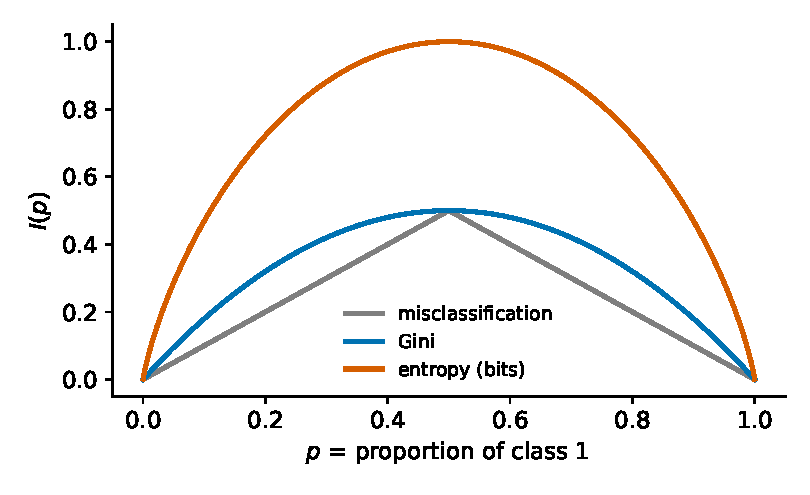
\includegraphics[height=0.55\textheight]{fig_impurity.pdf}
\end{center}
\vspace{-4pt}
All three are symmetric about $p=\tfrac12$, zero at the ends, maximal in the middle. Gini and entropy
are strictly concave; misclassification is concave but piecewise \emph{linear}. That difference matters.
\end{frame}

\begin{frame}{Concavity}\footnotesize
\begin{claim}{Gini and entropy are strictly concave on the simplex}
\end{claim}
\begin{derivation}{Binary case: check the second derivative}
\begin{align*}
I_G(p)&=2p-2p^2, & I_G''(p)&=-4<0 .\\
I_H(p)&=-p\log_2p-(1-p)\log_2(1-p), & I_H''(p)&=-\frac{1}{\ln2}\Bigl(\frac1p+\frac1{1-p}\Bigr)<0 .
\end{align*}
\end{derivation}
\begin{derivation}{General $K$}
Gini: $I_G(\vp)=1-\vp\T\vp$ has Hessian $-2\vI\prec0$. \quad
Entropy: $\partial^2I_H/\partial p_k\partial p_l=-\delta_{kl}/(p_k\ln2)$, a negative diagonal matrix.
\end{derivation}
\begin{keypoint}
Misclassification $\min(p,1-p)$ is concave too, but with $I''=0$ except at $p=\tfrac12$. It cannot tell
apart two splits that move the same number of points across the majority line. Next slide.
\end{keypoint}
\end{frame}

\begin{frame}{Information Gain}\small
Split node $S$ (proportions $\vp$, $N$ points) into children $S_L,S_R$ (proportions $\vp_L,\vp_R$; $N_L+N_R=N$).
\begin{block}{Gain of a split}
\[
\Delta=I(\vp)-\Bigl[\frac{N_L}{N}I(\vp_L)+\frac{N_R}{N}I(\vp_R)\Bigr]
\]
\end{block}
\begin{claim}{$\Delta\ge0$ for any concave $I$, with equality iff $\vp_L=\vp_R$ when $I$ is strictly concave}
\end{claim}
\begin{derivation}{Proof}
The parent's proportions are the weighted average of the children's:
$\vp=\frac{N_L}{N}\vp_L+\frac{N_R}{N}\vp_R$ (count the points of each class). Jensen's inequality for concave $I$
with weights $w_L=N_L/N$, $w_R=N_R/N$:
\[
I\bigl(w_L\vp_L+w_R\vp_R\bigr)\ \ge\ w_LI(\vp_L)+w_RI(\vp_R),
\]
which is exactly $\Delta\ge0$. Strict concavity gives strict inequality unless $\vp_L=\vp_R$. \qed
\end{derivation}
A split never increases impurity. It fails to decrease it only when both children look like the parent.
\end{frame}

\begin{frame}{Why Not Split on Misclassification Error?}\small
Parent: $400$ positives, $400$ negatives. Two candidate splits:
\begin{center}
\begin{tabular}{lcccc}
\toprule
 & left child & right child & misclass.\ after & Gini after \\
\midrule
Split A & $(300,100)$ & $(100,300)$ & $\frac{100+100}{800}=0.250$ & $\frac{400}{800}\cdot0.375+\frac{400}{800}\cdot0.375=0.375$ \\[3pt]
Split B & $(200,400)$ & $(200,0)$ & $\frac{200+0}{800}=0.250$ & $\frac{600}{800}\cdot0.444+\frac{200}{800}\cdot0=0.333$ \\
\bottomrule
\end{tabular}
\end{center}
\vspace{4pt}
\begin{itemize}
  \item Misclassification: both splits leave $200$ errors. Tie. It does not care that B produced a \emph{pure} leaf.
  \item Gini: B scores $0.333<0.375$. B wins, because a pure child is worth something even if the other child got worse.
  \item Entropy agrees with Gini ($0.811$ vs $0.689$ bits).
\end{itemize}
\begin{keypoint}
Splits are chosen for what they enable \emph{later}. A pure leaf is done; a $(300,100)$ leaf still needs work.
Strictly concave impurities see this; the piecewise-linear one does not. Gini and entropy are used for growing;
misclassification is used for pruning and reporting.
\end{keypoint}
% verify: L4.gini_vs_misclass
\end{frame}

\begin{frame}{Numerical Example: One Split, Three Criteria}\footnotesize
Parent $S$: $8$ positives, $4$ negatives. Split into $S_L=(6,1)$ and $S_R=(2,3)$.
\begin{derivation}{Entropy}
\begin{align*}
I_H(S)&=-\tfrac{8}{12}\log_2\tfrac{8}{12}-\tfrac{4}{12}\log_2\tfrac{4}{12}=0.9183\\
I_H(S_L)&=-\tfrac67\log_2\tfrac67-\tfrac17\log_2\tfrac17=0.5917,\qquad
I_H(S_R)=-\tfrac25\log_2\tfrac25-\tfrac35\log_2\tfrac35=0.9710\\
\Delta_H&=0.9183-\bigl[\tfrac{7}{12}(0.5917)+\tfrac{5}{12}(0.9710)\bigr]=0.9183-0.7498=0.1685\ \text{bits}
\end{align*}
\end{derivation}
\begin{derivation}{Gini}
\[
I_G(S)=1-\tfrac{64+16}{144}=0.4444,\quad I_G(S_L)=1-\tfrac{36+1}{49}=0.2449,\quad I_G(S_R)=1-\tfrac{4+9}{25}=0.4800
\]
\[
\Delta_G=0.4444-\bigl[\tfrac{7}{12}(0.2449)+\tfrac{5}{12}(0.4800)\bigr]=0.4444-0.3429=0.1016 .
\]
\end{derivation}
\begin{derivation}{Misclassification}
\[
I_M(S)=\tfrac{4}{12},\quad I_M(S_L)=\tfrac17,\quad I_M(S_R)=\tfrac25,\quad
\Delta_M=\tfrac{4}{12}-\bigl[\tfrac{7}{12}\cdot\tfrac17+\tfrac{5}{12}\cdot\tfrac25\bigr]=\tfrac{4}{12}-\tfrac{3}{12}=0.0833 .
\]
\end{derivation}
% verify: L4.information_gain_example
\end{frame}

% =============================================================================
\sectionframe{Growing and Pruning}
% =============================================================================

\begin{frame}{Top-Down Greedy Training (CART)}\small
\begin{algorithm}[H]
\SetAlgoLined
\SetKwFunction{Grow}{Grow}
\SetKwProg{Fn}{Function}{:}{}
\Fn{\Grow{$S$}}{
  \If{stopping rule holds for $S$}{\Return leaf with $\hat c=\bar y_S$ or $\argmax_k\hat p_k$}
  \ForEach{feature $j$ and threshold $s$ among the midpoints of sorted $x_{ij}$}{
    $S_L\gets\{i\in S:x_{ij}\le s\}$, \ $S_R\gets S\setminus S_L$\;
    $\Delta(j,s)\gets I(S)-\bigl[\tfrac{|S_L|}{|S|}I(S_L)+\tfrac{|S_R|}{|S|}I(S_R)\bigr]$\;
  }
  $(j^\star,s^\star)\gets\argmax\Delta(j,s)$\;
  \Return node asking ``$x_{j^\star}\le s^\star$?'' with children \Grow{$S_L$}, \Grow{$S_R$}\;
}
\end{algorithm}
\begin{itemize}
  \item Cost per node: sort each feature once, $O(pN\log N)$, then a linear scan per feature updates the class counts
        incrementally. A full tree of depth $d$: $O(d\,pN\log N)$.
  \item Categorical features with $q$ levels: $2^{q-1}-1$ possible subsets. For binary $y$, sort levels by
        $\hat p$ and only $q-1$ splits need checking (Breiman et al., 1984). Regression: same, sort by $\bar y$.
  \item Missing values: send them down a \emph{surrogate} split, or treat ``missing'' as a category.
\end{itemize}
\end{frame}

\begin{frame}{When to Stop}\footnotesize
A tree grown until every leaf is pure has zero training error and memorizes the noise.
Stopping rules are the tree's regularizers:
\begin{itemize}
  \item \textbf{Maximum depth} $d_{\max}$ --- at most $2^{d_{\max}}$ leaves.
  \item \textbf{Minimum samples per leaf} $n_{\min}$ --- each leaf's $\hat c$ is an average of at least $n_{\min}$ labels,
        so its variance is at most $\sigma^2/n_{\min}$.
  \item \textbf{Minimum gain} $\Delta_{\min}$ --- do not split for less than this. Dangerous: a useless split can enable
        a very good one below it (XOR is the standard example).
\end{itemize}
\vspace{4pt}
\begin{block}{Cost-complexity pruning (Breiman)}
Grow a large tree $T_0$. For $\alpha\ge0$, find the subtree $T\subseteq T_0$ minimizing
\[
C_\alpha(T)=\sum_{m=1}^{|T|}N_m\,I(R_m)+\alpha\,|T| ,
\]
training impurity plus a charge per leaf. Larger $\alpha$: smaller tree. The minimizing subtrees are nested as
$\alpha$ grows, so the whole path is computed by repeatedly collapsing the internal node with the smallest
increase in impurity per leaf removed (\emph{weakest link}). Choose $\alpha$ by cross-validation.
\end{block}
\end{frame}

\begin{frame}{Regression Trees}
Same algorithm with the variance of $y$ as impurity:
\[
I(S)=\frac{1}{|S|}\sum_{i\in S}(y_i-\bar y_S)^2,\qquad
\Delta(j,s)=I(S)-\Bigl[\tfrac{|S_L|}{|S|}I(S_L)+\tfrac{|S_R|}{|S|}I(S_R)\Bigr].
\]
\begin{derivation}{Maximizing $\Delta$ is minimizing the RSS after the split}
$|S|\,I(S)$ is the RSS of predicting $\bar y_S$ on $S$. So
$|S|\Delta=\RSS(S)-\bigl[\RSS(S_L)+\RSS(S_R)\bigr]$, and $\RSS(S)$ does not depend on the split.
Maximizing $\Delta$ over $(j,s)$ is minimizing $\RSS(S_L)+\RSS(S_R)$: the best split is the one whose two
constant fits explain the most.
\end{derivation}
\begin{itemize}
  \item Predictions are means of training responses, so a regression tree \textbf{cannot extrapolate}: outside
        the range of the training $y$, it is silent.
  \item The fitted function is a staircase. Smooth targets need many leaves; bagging (next) smooths the staircase.
\end{itemize}
\end{frame}

\begin{frame}{Trees Are High-Variance}
\begin{center}
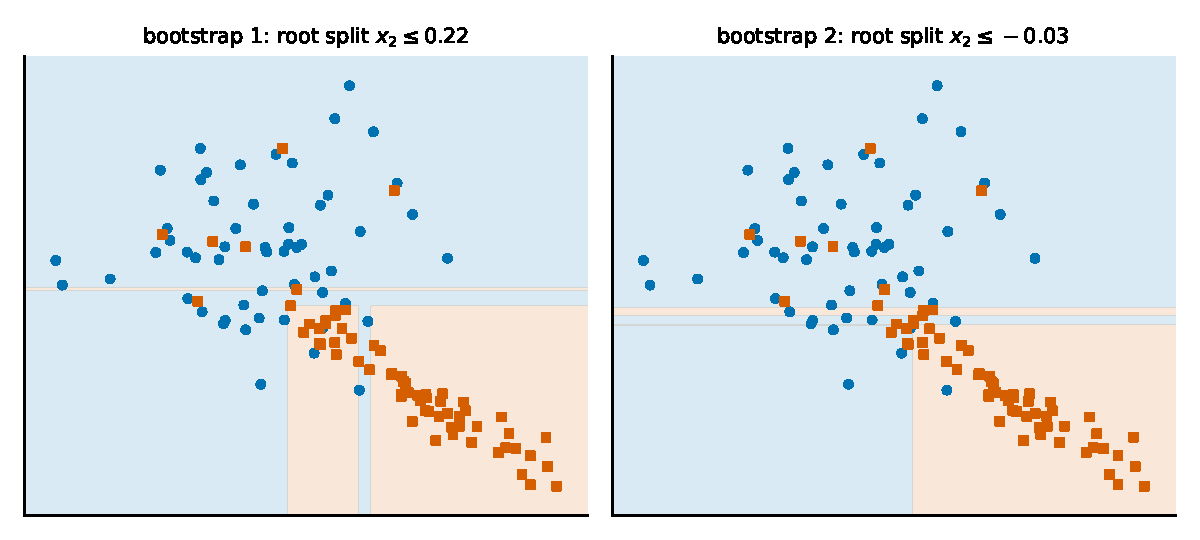
\includegraphics[height=0.5\textheight]{fig_tree_instability.pdf}
\end{center}
\vspace{-4pt}
Two trees fitted to two bootstrap resamples of the same data. The top split changed; everything below it
changed with it. In the language of Lecture 1: a deep tree has \textbf{low bias} (it can represent almost any
function of the inputs) and \textbf{high variance} (which function it picks depends heavily on the sample).
\end{frame}

% =============================================================================
\sectionframe{Bagging}
% =============================================================================

\begin{frame}{Averaging Reduces Variance}\footnotesize
Lecture 1's decomposition says variance is the price of low bias. Averaging is the tool for variance.
\begin{claim}{$B$ predictors, each with variance $\sigma^2$, pairwise correlation $\rho$}
\[
\Var\Bigl(\frac1B\sum_{b=1}^B\hat f_b(\vx)\Bigr)=\rho\,\sigma^2+\frac{1-\rho}{B}\,\sigma^2 .
\]
\end{claim}
\begin{derivation}{Proof}
\begin{align*}
\Var\Bigl(\frac1B\sum_b\hat f_b\Bigr)&=\frac1{B^2}\Bigl[\sum_b\Var(\hat f_b)+\sum_{b\ne b'}\Cov(\hat f_b,\hat f_{b'})\Bigr]
=\frac1{B^2}\Bigl[B\sigma^2+B(B-1)\rho\sigma^2\Bigr]\\
&=\frac{\sigma^2}{B}+\frac{B-1}{B}\rho\sigma^2
=\rho\sigma^2+\frac{1-\rho}{B}\sigma^2 . \qquad\qed
\end{align*}
\end{derivation}
\begin{keypoint}
As $B\to\infty$ the second term vanishes and the first does not. Averaging can drive variance down to
$\rho\sigma^2$, no further. Everything depends on making the predictors \emph{different} from one another.
\end{keypoint}
\end{frame}

\begin{frame}{The Variance Floor}
\begin{center}
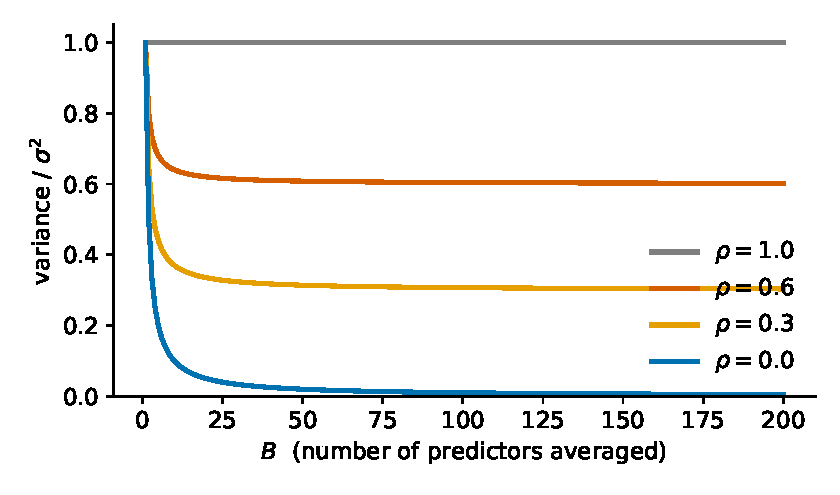
\includegraphics[height=0.5\textheight]{fig_bagging_variance.pdf}
\end{center}
\vspace{-4pt}
$\rho=1$: identical predictors, averaging does nothing. $\rho=0$: independent, variance $\to0$ like $1/B$.
Real bagged trees sit in between --- they are fitted to overlapping data --- so the curve flattens at $\rho\sigma^2$.
\end{frame}

\begin{frame}{Bootstrap Aggregating (Breiman, 1996)}
We have one sample, not $B$. Manufacture $B$ by resampling:
\begin{algorithm}[H]
\SetAlgoLined
\For{$b=1,\dots,B$}{
  draw $\Dset^{(b)}$: $N$ points from $\Dset$ \emph{with replacement}\;
  fit a deep tree $\hat f_b$ to $\Dset^{(b)}$ (no pruning)\;
}
\KwOut{$\hat f_{\text{bag}}(\vx)=\frac1B\sum_b\hat f_b(\vx)$ \ (regression) \ or majority vote / averaged proportions (classification)}
\end{algorithm}
\begin{itemize}
  \item Each $\hat f_b$ has the same distribution, so $\E[\hat f_{\text{bag}}]=\E[\hat f_1]$: \textbf{bias is unchanged}.
        Use deep trees --- low bias --- and let the average handle the variance.
  \item The bootstrap samples overlap, so $\rho>0$. Typical values for trees: $\rho\in[0.3,0.6]$.
  \item More trees never hurt: variance is non-increasing in $B$. $B=100$--$500$ is usual; the curve flattens.
\end{itemize}
\end{frame}

\begin{frame}{Out-of-Bag Error: Cross-Validation for Free}
\begin{derivation}{How much of the data does each tree see?}
The probability that a given point is \emph{not} drawn in one of $N$ draws with replacement is
\[
\Bigl(1-\frac1N\Bigr)^N\ \xrightarrow[N\to\infty]{}\ e^{-1}\approx0.368 .
\]
(Take logs: $N\log(1-1/N)=N(-1/N-1/(2N^2)-\dots)\to-1$.)
\end{derivation}
So each tree is fitted on about $63\%$ of the distinct points, and about $37\%$ are \textbf{out of bag} for it.
\begin{itemize}
  \item For each $\vx_i$, average only the trees that did not see it: $\hat f_{\text{oob}}(\vx_i)$. Roughly $B/3$ trees.
  \item The error of $\hat f_{\text{oob}}$ on the training set is an honest estimate of test error --- every prediction
        is made by trees that never saw the point. No folds, no refitting.
  \item OOB error tracks the CV error of a bagged ensemble closely and costs nothing extra.
\end{itemize}
\end{frame}

\begin{frame}{Random Forests (Breiman, 2001)}
Bagging's floor is $\rho\sigma^2$. Lower $\rho$ by making the trees see different \emph{features}, not just
different rows:
\begin{block}{The one change}
At every split, choose the best split among a random subset of $m$ of the $p$ features (fresh subset each node).
Defaults: $m=\lfloor\sqrt p\rfloor$ for classification, $m=\lfloor p/3\rfloor$ for regression.
\end{block}
\begin{itemize}
  \item A dominant feature no longer appears at the top of every tree. Trees become less alike: $\rho$ drops.
  \item Each tree gets slightly worse (higher $\sigma^2$, some bias); the ensemble gets better. The trade is
        governed by $\rho\sigma^2$, and $\rho$ falls faster than $\sigma^2$ rises.
  \item $m=p$ recovers bagging. $m=1$ chooses the feature at random and only optimizes the threshold.
\end{itemize}
\begin{keypoint}
Random forests do not overfit as $B$ grows: the variance of the average is monotone in $B$ and bounded below
by $\rho\sigma^2$. They \emph{can} overfit through the depth of the individual trees.
\end{keypoint}
\end{frame}

\begin{frame}{Bagging and Forests in Practice}
\begin{center}
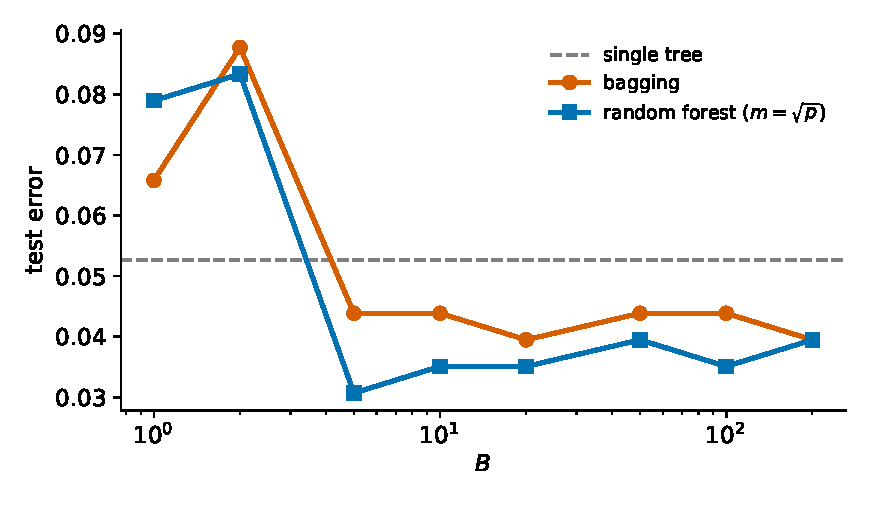
\includegraphics[height=0.5\textheight]{fig_ensemble_error.pdf}
\end{center}
\vspace{-4pt}
Test error against $B$ on a benchmark. A single tree (dashed) is the $B=1$ value. Bagging drops quickly then
flattens; the forest flattens lower. Neither curve turns back up.
\end{frame}

\begin{frame}{Which Features Matter?}
Trees make the question answerable:
\begin{itemize}
  \item \textbf{Mean decrease in impurity.} Sum, over every node that splits on feature $j$, the gain $\Delta$
        weighted by the node size; average over trees. Fast, but biased toward features with many distinct values.
  \item \textbf{Permutation importance.} Shuffle column $j$ in the OOB data and measure how much OOB error rises.
        Model-agnostic and unbiased in the above sense; costs one pass per feature.
\end{itemize}
\vspace{4pt}
\begin{caution}
Importance measures association with the prediction, not causation, and they split credit arbitrarily among
correlated features. Two copies of the same column each get half the importance.
\end{caution}
\end{frame}

% =============================================================================
\sectionframe{Summary}
% =============================================================================

\begin{frame}{What We Proved Today}
\begin{enumerate}
  \item Leaf values: the mean (regression) or the majority (classification) minimize the empirical risk on the leaf.
  \item Gini and entropy are strictly concave; misclassification is only piecewise linear.
  \item Gain $\Delta\ge0$ for any concave impurity, by Jensen; strict when children differ. A strictly concave
        impurity rewards pure children even when the error count does not move.
  \item Regression trees maximize the reduction in RSS. Leaves cannot extrapolate.
  \item $\Var(\text{average of }B)=\rho\sigma^2+\tfrac{1-\rho}{B}\sigma^2$: bagging removes the second term and
        leaves the first; random forests attack the first by lowering $\rho$.
  \item Each bootstrap sample omits $\approx e^{-1}$ of the data, which gives an honest out-of-bag error.
\end{enumerate}
\end{frame}

\begin{frame}{Next}
\textbf{Lecture 5 (Monday)} --- the other way to combine trees: boosting. Instead of averaging many
independent low-bias models, add many dependent high-bias models one at a time. Functional gradient descent,
AdaBoost and its training-error bound, and why it keeps improving after the training error hits zero.
\vspace{8pt}

\textbf{Lab 3 (Wednesday, Rodrigo)} --- information gain by hand, \texttt{min\_samples\_leaf} and overfitting,
bagging vs.\ random forest vs.\ boosting on one dataset, and tuning all three.
\vspace{8pt}

\textbf{Reading} --- \emph{ESL} \S9.2 (trees), \S8.7 (bagging), \S15.1--15.3 (random forests).
Breiman (2001), \emph{Random Forests}, Machine Learning 45.
\end{frame}

\end{document}
